\documentclass[11pt,a4paper]{article}

\usepackage{booktabs}
\usepackage{graphicx}
\usepackage{longtable}
\usepackage{listings}
\usepackage{xcolor}
\lstset{
  basicstyle=\small\ttfamily,
  backgroundcolor=\color{gray!10},
  frame=single,
  rulecolor=\color{gray!40},
  breaklines=true,
  columns=fullflexible,
}
\usepackage[colorlinks=true,linkcolor=blue,urlcolor=blue,citecolor=blue]{hyperref}
\usepackage{geometry}
\geometry{margin=1in}

\title{Response to Reviewer Comments}
\author{}
\date{}

\begin{document}
\maketitle
\setcounter{tocdepth}{2}
\tableofcontents
\newpage

% ============================================================================
\section{Response to Reviewer \#1}
% ============================================================================

% ----------------------------------------------------------------------------
\subsection{Comment 1.1 and 1.6--- Anomaly Backtracking Logic \textbf{[COMPLETED]}}

\subsubsection{Comment}

\begin{enumerate}
  \item \textbf{Comment 1.1}``The framework claims to reduce `hallucinations,' but it does not clearly explain how the `Anomaly Backtracking' logic works in the architecture section.''

  \item \textbf{Comment 1.6}``The paper should include a clear, step-by-step description of how the PM-Agent detects a failure in the TE-Agent and triggers a state transition back to either the ME-Agent or the PY-Agent.''
\end{enumerate}

\subsubsection{Response}
We thank the reviewer for pointing out this ambiguity. We agree that the original manuscript did not make the failure-triggering and backtracking chain sufficiently explicit. We have therefore revised Section 3.2 to distinguish (i) controller-level execution/verification failure detection in Step 6 from (ii) PM-Agent-led diagnosis and stack-based backtracking in Step 7. In the SOP-MAS framework, exception backtracking is triggered whenever the post-generation execution or verification stage fails and \texttt{is\_backward=True}; therefore, its activation does not depend on whether the TE-Agent has been selected in the current forward pass.

More specifically, when the collaboration budget $K$ is large enough to include the TE-Agent, the TE-Agent performs an additional execution/testing step and provides more structured diagnostic evidence, such as execution results and solver logs, which helps localize the error source more precisely during backtracking. When $K$ is smaller and the TE-Agent is not selected, the framework can still trigger stack-based backtracking based on the global failure signal. In that case, previously selected agents are queried in reverse order to judge whether their outputs caused the failure and to refine them if necessary, although the available error information is coarser than in the TE-Agent-assisted case.

We further clarify that the transition to the PY-Agent or ME-Agent is not implemented as a hard-coded branch on TE-Agent error types. Instead, the PM-Agent queries agents in reverse workflow order, so code-level defects are typically localized first to the PY-Agent, whereas failures that persist beyond code correction propagate further to the ME-Agent for model-level revision. We have revised the manuscript accordingly to make this trigger chain explicit and to clarify that the TE-Agent enhances error diagnosis, rather than serving as the sole trigger of anomaly backtracking.

For clarity, we summarize the two representative settings below.

\begin{enumerate}
\item \textbf{$K=4$: DE-Agent $\rightarrow$ ME-Agent $\rightarrow$ PY-Agent $\rightarrow$ TE-Agent.} Step 6 receives both the global execution/verification failure signal and the TE-Agent runtime report. The PM-Agent then triggers Step 7, backtracks in reverse order, typically queries the PY-Agent first, and continues to the ME-Agent only if the failure is not resolved at the code level.

\item \textbf{$K=3$: DE-Agent $\rightarrow$ ME-Agent $\rightarrow$ PY-Agent.} The TE-Agent is not selected, so Step 6 returns only the global execution/verification failure signal. Even so, the PM-Agent still triggers the same reverse-order backtracking in Step 7, typically starting from the PY-Agent and propagating to the ME-Agent if necessary, but with coarser diagnostic evidence.
\end{enumerate}

\subsubsection{Modifications}
\begin{enumerate}
\item \textbf{Section 3.1, Agent Definition (L277) --- MODIFY}
\begin{quote}
\textbf{Before:} ``\textit{The TE-Agent \ldots{} carries out the execution of the code within a sandbox environment \ldots{} and subsequently provide a report on the execution.}''\\[4pt]
\textbf{After:} ``\textit{\textcolor{red}{The TE-Agent was redefined as a supplementary testing and fine-grained diagnosis module. Controller-level code execution and verification remain framework responsibilities, while the TE-Agent contributes structured diagnostic artifacts such as execution summaries, test cases, and solver logs to support failure localization during backtracking.}}'' 
\end{quote}

\item \textbf{Section 3.2, Step 6--7 (L325--335) --- MODIFY}
\begin{quote}
\textbf{Before:} ``\textit{If the TE-Agent is activated, it executes the code generated by the PY-Agent \ldots{} Only when both automated checks and expert sign-off are satisfied does the workflow advance to Step~7. Otherwise, proceed to Step~7 for exception backtracking. When an execution error is detected and \texttt{is\_backward} = \texttt{True}, trigger the backtracking mechanism.}''\\[4pt]
\textbf{After:} ``\textit{\textcolor{red}{After the $K$-step forward pass, the framework executes the latest solver code and performs a global verification check. If the TE-Agent is activated, it additionally executes the code generated by the PY-Agent and provides a structured runtime report, thereby supplying finer-grained diagnostic evidence. If the execution and verification stage succeeds, the workflow proceeds directly to Step~8. Otherwise, if \texttt{is\_backward} = \texttt{True}, the PM-Agent triggers Step~7 for exception backtracking; if \texttt{is\_backward} = \texttt{False}, the workflow skips backtracking and terminates with the current failure outcome. When backtracking is triggered, the PM-Agent pops the stack in reverse order and queries previously selected agents one by one; if the TE-Agent was selected, its structured execution report is used as part of the diagnostic evidence, whereas otherwise the diagnosis relies on the coarser global failure signal. Because the forward workflow follows the monotonic order DE-Agent $\rightarrow$ ME-Agent $\rightarrow$ PY-Agent $\rightarrow$ TE-Agent, implementation-level defects are typically examined first at the PY-Agent, whereas failures that persist beyond code correction are propagated further to the ME-Agent for model-level revision.}}'' 
\end{quote}

\item \textbf{Section 3.3, Item 3 (L351) --- MODIFY}
\begin{quote}
\textbf{Before:} ``\textit{Upon the occurrence of an exception during code execution within the sandbox environment, the TE-Agent retains the error information in the shared message pool.}''\\[4pt]
\textbf{After:} ``\textit{\textcolor{red}{Upon the occurrence of an execution or verification failure, the framework records the failure signal in the shared message pool. When selected, the TE-Agent additionally contributes a dedicated execution report containing finer-grained diagnostic evidence.}}'' 
\end{quote}

\item \textbf{Section 4.2, Group 4 description and discussion (L460, L484) --- MODIFY}
\begin{quote}
\textbf{Before:} ``\textit{However, the exception backtracking mechanism remains active, enabling each agent to perform self-checks on its output to detect probable errors. \ldots{} Group 4 indicates that the exclusion of the TE-Agent still results in a relatively high accuracy, as the testing agent is capable of providing detailed error information, and errors can be rectified via the exception-backtracking mechanism.}''\\[4pt]
\textbf{After:} ``\textit{\textcolor{red}{However, the exception backtracking mechanism remains active because it is triggered by controller-level execution or verification failure rather than by TE-Agent selection itself. In this setting, previously selected agents are queried in reverse order based on a coarser global failure signal. \ldots{} Group 4 indicates that the exclusion of the TE-Agent still results in a relatively high accuracy because exception backtracking remains available even without the dedicated testing module, although error localization then relies on coarser global failure feedback rather than on the structured execution report normally produced by the TE-Agent.}}'' 
\end{quote}
\end{enumerate}

% ----------------------------------------------------------------------------
\subsection{Comment 1.2 and 1.7 --- Temperature Settings \textbf{[COMPLETED]}}

\subsubsection{Comment}

\begin{enumerate}
  \item \textbf{Comment 1.2: }``The framework relies on specific large language models (LLMs), like GPT-4, but it does not explore how changing temperature settings ($t_i$) affects its performance.''

  \item \textbf{Comment 1.7: }``The paper should add an experiment that changes the LLM temperature ($t_i$) and \texttt{top\_p} values to show how stable the generated Mixed Integer Programming (MIP) formulations are.''
\end{enumerate}

\subsubsection{Response}
This comment overlaps substantially with Comment~1.2 and is therefore addressed jointly there. We thank the reviewer for this observation. We wish to clarify that Section~4.2 already presents a comprehensive sensitivity analysis examining the effect of temperature on framework performance. Specifically, a grid search was performed over $t_{ME}, t_{PY} \in [0.2, 0.4, 0.8, 1.0]$ while varying $K \in [2,5]$, using AR as the evaluation metric. The results, presented in Figure~3, demonstrate that lower temperatures consistently yield higher accuracy for both the ME-Agent and PY-Agent.

Regarding the scope of temperature coverage, we focused on $t_{ME}$ and $t_{PY}$ because these two agents are directly responsible for mathematical model construction and executable code generation, respectively, which are the primary determinants of solution accuracy. The temperatures of the remaining agents have a relatively minor impact for different reasons: the DE-Agent performs structured data extraction whose output format is largely determined by the input schema; the PM-Agent's selection strategy is constrained by the sub-sequence rules, which limits the effect of temperature-induced randomness; and the TE-Agent and BA-Agent do not directly affect model accuracy, as validated by the ablation study in Section~4.3 (Group~2 and Group~4).

Concerning the $\texttt{top\_p}$ parameter raised jointly in Comment~1.7, it is maintained at its default value throughout all experiments. Since $\texttt{top\_p}$ and temperature are correlated mechanisms for controlling LLM output randomness, varying temperature alone is sufficient to capture the effect of stochasticity on framework performance without exponentially increasing the experimental dimension. This practice is consistent with prior work in the same domain, such as Chain-of-Experts (CoE)~[Xiao et al., 2023], where only temperature is tuned.

Regarding MIP formulation stability across runs, we acknowledge that variable naming and symbolic representation inevitably differ across runs due to the inherent stochasticity of LLM generation. However, such differences are cosmetic and do not affect mathematical equivalence. For structural consistency: when exception backtracking is enabled (\texttt{is\_backward}~=~\texttt{True}), the verification--backtracking loop corrects formulation errors based on ground-truth comparison, so the final formulation reliably converges to a correct model. When backtracking is disabled (\texttt{is\_backward}~=~\texttt{False}), structural inconsistency across runs is possible---a model may use a different constraint set or modeling approach while still yielding the correct optimal objective value. The sensitivity analysis in Section~4.2 was conducted under \texttt{is\_backward}~=~\texttt{False} to isolate the effect of temperature; the resulting AR values therefore reflect single-pass generation reliability rather than post-correction consistency.

We have revised Section~4.2 to (1)~explicitly justify the focus on $t_{ME}$ and $t_{PY}$, (2)~state that $\texttt{top\_p}$ is kept at its default value, and (3)~correct an inconsistency in Step~6 where the verification criterion allowed a Feasible status, which has been tightened to require an Optimal status to align with the AR definition in Section~4.1.

\subsubsection{Modifications}
\begin{enumerate}
\item \textbf{Section 4.2, Sensitivity Analysis (L430) --- MODIFY (restructure and merge two paragraphs into one)}
\begin{quote}
\textbf{Before:} ``\textit{Within the SOP-MAS framework, pivotal parameters encompass the maximum collaboration count $K$ of the PM-Agent, alongside the temperatures of the ME-Agent and PY-Agent, denoted as $t_{ME}$ and $t_{PY}$, respectively. The parameter $K$ exerts influence over the overall depth and breadth of the workflow by modulating the number of agent invocations. Temperature significantly affects the optimization modeling and solution outputs generated by the agents. Specifically, elevated temperatures foster the development of more innovative solutions, while reduced temperatures bolster deterministic reasoning, and in consequence ensuring stability and compliance of the outputs. This trade-off between precision and creativity mandates meticulous calibration of the temperature parameters tailored to specific task scenarios. [paragraph break] Among all agents, the temperatures of the ME-Agent and PY-Agent are prioritized for sensitivity analysis because\dots}''\\[4pt]
\textbf{After:} ``\textit{\textcolor{red}{Within the SOP-MAS framework, the maximum collaboration count $K$ of the PM-Agent governs the depth and breadth of the workflow by modulating the number of agent invocations. Among the six agents, the temperatures of the ME-Agent and PY-Agent, denoted as $t_{ME}$ and $t_{PY}$, are the primary determinants of solution accuracy, because these two agents are directly responsible for mathematical model construction and executable code generation, respectively. The temperatures of the remaining agents (DE-Agent, PM-Agent, TE-Agent, and BA-Agent) have a relatively minor impact on the optimization outcome, as validated by the ablation study in Section~4.3. Temperature significantly affects the optimization modeling and solution outputs generated by the agents: elevated temperatures foster more innovative solutions, while reduced temperatures bolster deterministic reasoning, ensuring stability and compliance of the outputs. This trade-off between precision and creativity mandates meticulous calibration of the temperature parameters tailored to specific task scenarios.}}''
\end{quote}

\item \textbf{Section 3.2, Step 6 (L315) --- MODIFY}
\begin{quote}
\textbf{Before:} ``\textit{The solution is deemed correct only if (i) the solver status is Optimal or Feasible, and (ii) the objective value matches the ground-truth optimum.}''\\[4pt]
\textbf{After:} ``\textit{\textcolor{red}{The solution is deemed correct only if (i) the solver reports an Optimal status, and (ii) the objective value matches the ground-truth optimum.}}''
\end{quote}
\end{enumerate}

% ----------------------------------------------------------------------------
\subsection{Comment 1.3 --- Multi-Agent Interaction Latency vs.\ Manual Modeling}

\subsubsection{Comment}
``There is not enough discussion about the delay caused by the multi-agent interaction layers compared to traditional manual modeling timelines.''

\subsubsection{Response}

\subsubsection{Modifications}


% ----------------------------------------------------------------------------
\subsection{Comment 1.4 --- BA-Agent User Study Data}

\subsubsection{Comment}
``The claim that the system reduces barriers for non-experts lacks user-study data to support the effectiveness of the `Business Analyst Agent.' ''

\subsubsection{Response}

\subsubsection{Modifications}

% ----------------------------------------------------------------------------
\subsection{Comment 1.5 --- ECR paper Citation \textbf{[COMPLETED]}}

\subsubsection{Comment}
``In Section 2.4 (Challenges). It is suggested to refer from the paper: `A novel permissioned blockchain approach for scalable and privacy-preserving IoT authentication'. This citation addresses privacy and trust issues in decentralized environments, which is important for discussing the security of data shared between port agents in the ECR network.''

\subsubsection{Response}
[Completed, no modifications needed]

\subsubsection{Modifications}
\begin{enumerate}
\item \textbf{Section 2.4 (L253) --- ADD}
\begin{quote}
\textbf{After:} ``\textit{\textcolor{red}{. This decentralized nature of ECR networks, where sensitive operational data (e.g., container inventories and transport schedules) must be shared across organizational boundaries, underscores the importance of privacy-preserving and trust mechanisms for effective multi-stakeholder collaboration} \textcolor{red}{[\texttt{27}]}}''\end{quote}
\end{enumerate}


% ----------------------------------------------------------------------------
\subsection{Comment 1.8 --- Terminology Consistency \textbf{[COMPLETED]}}

\subsubsection{Comment}
``The terminology must be consistent; the terms `SOP-MAS' and `LLM-agent system' should be used in the same way throughout.''

\subsubsection{Response}
A comprehensive terminology audit was performed. ``LLM-agent system'' did not appear in the original text. We have unified the framework reference as \textbf{SOP-MAS} throughout the paper: (1)~the acronym is formally introduced in the Abstract upon first mention; (2)~all subsequent framework references use ``SOP-MAS'' or ``the SOP-MAS framework'' instead of informal paraphrases; (3)~``SOP-MAS system'' redundancy is removed. The generic terms ``multi-agent system'' and ``MAS'' are reserved for the general concept in the literature review.

\subsubsection{Modifications}
\begin{enumerate}
\item \textbf{Abstract (L172) --- MODIFY}
\begin{quote}
\textbf{Before:} ``\textit{by designing a multi-agent collaborative framework grounded in artificial intelligence large language models. This framework interprets \ldots}''\\[4pt]
\textbf{After:} ``\textit{by designing \textcolor{red}{SOP-MAS (Standard Operating Procedure--Multi-Agent System), a multi-agent collaborative framework grounded in artificial intelligence large language models. This framework} interprets \ldots}''
\end{quote}

\item \textbf{Methodology Section (L267) --- MODIFY}
\begin{quote}
\textbf{Before:} ``\textit{This research proposes a specialized LLM-based MAS framework predicated upon the Standardized Operating Procedure (SOP) paradigm.}''\\[4pt]
\textbf{After:} ``\textit{\textcolor{red}{This section details the SOP-MAS framework, which is predicated upon the Standardized Operating Procedure (SOP) paradigm.}}''
\end{quote}

\item \textbf{Section 4.2 (L429) --- MODIFY}
\begin{quote}
\textbf{Before:} ``\textit{Within the framework of SOP-MAS system,}''\\[4pt]
\textbf{After:} ``\textit{\textcolor{red}{Within the SOP-MAS framework,}}''
\end{quote}
\end{enumerate}

\newpage
% ============================================================================
\section{Response to Reviewer \#2}
% ============================================================================

% ----------------------------------------------------------------------------
\subsection{Comment 2.A --- Precise Definition of ``Accuracy'' \textbf{[COMPLETED]}}

\subsubsection{Comment}
``Define `accuracy' precisely. Distinguish between successful code execution and reaching the global optimum (optimality gap). High-impact journals require measuring the mathematical quality of the solution, not just syntax.''

\subsubsection{Response}
We revised the AR definition to explicitly state the three-tier verification: compilation, solver optimality status, and ground-truth objective value matching. This is consistent with the verification criteria already described in Step~6 (Section 3.2).

\subsubsection{Modifications}
\begin{enumerate}
\item \textbf{Section 4.1 (L394) --- MODIFY}
\begin{quote}
\textbf{Before:} ``\textit{AR represents the proportion of codes that successfully satisfy all test cases.}''\\[4pt]
\textbf{After:} ``\textit{AR represents \textcolor{red}{the proportion of instances for which the generated code compiles, executes without runtime errors, the solver reports an Optimal status, and the resulting objective value matches the ground-truth optimum (optimality gap $= 0$)}.}''
\end{quote}
\end{enumerate}

% ----------------------------------------------------------------------------
\subsection{Comment 2.B --- Same LLM Backbone for All Baselines \textbf{[COMPLETED]}}

\subsubsection{Comment}
``Explicitly confirm if all baselines (OptiMUS, CoE, etc.) used the same DeepSeek-v3 backbone. Paradigm effectiveness cannot be validated if the underlying language models differ across comparisons.''

\subsubsection{Response}
We appreciate the reviewer's emphasis on comparison fairness, which we fully agree is essential for validating the paradigm. All baselines were evaluated under the same DeepSeek-v3-0324 backbone and identical hardware conditions to ensure a controlled comparison. Specifically, CoE and OptiMUS were reproduced using their publicly available code repositories (\url{https://github.com/xzymustbexzy/Chain-of-Experts} and \url{https://github.com/teshnizi/OptiMUS}, respectively) with the LLM configuration adapted to DeepSeek-v3-0324, while SPM and CoT were directly implemented following their published methodologies. The benchmark datasets and evaluation protocol (five runs per instance, $K=5$) were held constant across all methods. We have explicitly clarified this in Section 4.1.

\subsubsection{Modifications}
\begin{enumerate}
\item \textbf{Section 4.1 (L390) --- MODIFY}
\begin{quote}
\textbf{Before:} ``\textit{We adopt DeepSeek-v3-0324 as the backbone LLM, given its leading position among open weight models.}''\\[4pt]
\textbf{After:} ``\textit{We adopt DeepSeek-v3-0324 as the backbone LLM \textcolor{red}{for all methods}, given its leading position among open weight models.}''
\end{quote}

\item \textbf{Section 4.1 (L390) --- ADD}
\begin{quote}
\textbf{After:} ``\textit{\textcolor{red}{All baselines were evaluated under the same DeepSeek-v3-0324 backbone and identical hardware conditions to ensure a fair comparison.}}''
\end{quote}
\end{enumerate}

% ----------------------------------------------------------------------------
\subsection{Comment 2.C --- Equation (1) Probability Notation \textbf{[COMPLETED]}}

\subsubsection{Comment}
``Re-evaluate Equation 1's probabilistic notation. If agent selection is governed by deterministic prompts rather than actual probability distributions, simplify the math to avoid unnecessary `math-washing.' ''

\subsubsection{Response}
We appreciate the reviewer's scrutiny. Upon re-examination, we conclude that the probabilistic notation is justified. The PM-Agent does not use a hard-coded selection rule; instead, it determines the next agent via an LLM call with temperature $t_i > 0$, which introduces genuine stochasticity. The state $s$ passed to the LLM includes the problem description, message pool history, remaining selection quota, and the set of available agents, as shown in the PM-Agent's prompt template:

\begin{lstlisting}
# PROBLEM DESCRIPTION
Current optimization problem to solve: {problem_description}

# SELECTION CRITERIA
1. **STRICT ORDERING REQUIREMENT** (HIGHEST PRIORITY):
   - You MUST select agents in the order they appear in {agent_list}
   - The agent_id sequence MUST be monotonically increasing
   - NEVER skip agents or select out of order unless already selected

2. Available Options:
   - Already selected: {selected_agent_list}
   - Available pool: {allowed_agent_list}
   - Remaining quota: {remaining_collaborate_nums} / {max_collaborate_nums}

3. Selection Logic:
   - From {allowed_agent_list}, select the agent with the
     SMALLEST agent_id
\end{lstlisting}

This prompt structure maps directly to the state variables in $\pi_a(e|s) = Pr\{A_i=e \mid S_i=s\}$, where $s$ encodes the same information. Rather than removing the notation, we have added explicit definitions of all symbols to address Comment 3.3.

\subsubsection{Modifications}

\begin{enumerate}
\item \textbf{Section 3.2 Equation (1) (L309--310) --- ADD}
\begin{quote}
\textbf{After:} ``\textit{\textcolor{red}{where $s$ denotes the current state comprising the problem description, message pool history, remaining selection quota, and the set of available agents; $e$ is the candidate agent to be selected; and $A_i$ is the random variable representing the PM-Agent's selection at step $i$. The probability arises from the stochastic nature of LLM generation, since the PM-Agent determines the next agent via an LLM call rather than a hard-coded rule.}}''
\end{quote}
\end{enumerate}

% ----------------------------------------------------------------------------
\subsection{Comment 2.D --- Efficiency Metrics by Problem Size \textbf{[COMPLETED]}}

\subsubsection{Comment}
``Provide efficiency metrics correlated to problem size. Show how runtime and accuracy scale as the number of ports and time periods increase to prove industrial-grade scalability.''

\subsubsection{Response}
We appreciate the reviewer's concern regarding industrial-grade scalability. After careful analysis of the SOP-MAS workflow, we clarify that the framework's modeling runtime does not scale with problem size. The key insight lies in a deliberate architectural design: \textbf{problem description and concrete data are strictly separated}.

In SOP-MAS, the problem description $P$ (e.g., \texttt{description.txt}) is expressed in abstract symbolic form---parameters, variables, and constraints defined using index notation (e.g., $i \in I$ for ports, $t \in T$ for time periods)---while the concrete numerical data (e.g., port coordinates, demand matrices) resides in separate data files (e.g., \texttt{sample.json}). This separation is essential because embedding concrete data directly into the problem description would cause the text length to grow prohibitively with problem scale, overwhelming the LLM's context window and comprehension capacity. To illustrate this point, consider the following comparison:

\medskip
\noindent\textbf{Case A: Problem description with embedded data (not adopted).} If concrete data were embedded, even a simple 3-port ECR example would need to enumerate all values explicitly:

\begin{lstlisting}
# ECR Problem: 3 ports (A, B, C), T=1

The supply vector is S = [100, 50, 0] (TEU), where
  port A supplies 100 TEU, port B supplies 50 TEU, port C supplies 0 TEU.
The demand vector is D = [0, 0, 150] (TEU), where
  port A demands 0 TEU, port B demands 0 TEU, port C demands 150 TEU.
Unit transportation costs (CNY/TEU):
  c(A->B) = 2, c(A->C) = 10, c(B->C) = 3
  c(B->A) = 2, c(C->A) = 10, c(C->B) = 3
Storage cost h_i = 0, initial inventory I_i0 = 0.
  ... (for larger scale: 3 seaports + 5 dry ports + 7 time periods
   => text grows to O(|N|^2 * |T|) entries)
\end{lstlisting}

\noindent\textbf{Case B: Problem description with separated data (adopted by SOP-MAS).} The description uses abstract symbolic notation, remaining concise regardless of scale:

\begin{lstlisting}
# ECR Problem: Multi-period Network Flow Optimization

Network: Directed graph G=(N,E), where N = H (seaports) union L (dry ports).
Edges E represent repositioning routes: seaport-seaport,
seaport-dry port, and dry port-dry port.
Lambda_ij describes the hinterland relationship between seaport i
and dry port j.

Parameters:
- S_i^t: supply of empty containers at node i in period t
- D_i^t: demand at node i in period t
- c_ij: unit transport cost from node i to node j
- h_i: holding cost at node i
- U_i^max: storage capacity at node i
(Data provided separately in sample.json)
\end{lstlisting}

\noindent As shown, Case B's description length is independent of the number of ports or time periods, whereas Case A's text length grows proportionally to $O(|N|^2 \times |T|)$ as problem scale increases. For the Liaoning case with 3 seaports, 5 dry ports, and 7 time periods, Case A would require enumerating hundreds of specific values, whereas Case B's abstract description remains unchanged.

This design has the following implications for each step of the SOP process:

\begin{itemize}
\item \textbf{Steps 1--5 (Modeling):} Since $P$ remains fixed in length regardless of how many ports or time periods are involved, the DE-Agent's parameter extraction, the ME-Agent's model formulation, and the PY-Agent's code generation all produce identical outputs in terms of model structure and code template. The LLM API call time for these steps is therefore constant.

\item \textbf{Step 6 (Execution):} The TE-Agent executes the generated code via \texttt{optimize(data)}, where concrete data is loaded from external files. Only at this stage does the actual problem scale manifest, affecting the solver's runtime. Increasing the number of ports or time periods increases the number of decision variables and constraints fed to the solver, but the solver code template itself remains unchanged.

\item \textbf{Scalability implication:} The modeling overhead of SOP-MAS (Steps 1--5) is bounded by the sub-minute LLM API call time and is independent of problem scale. The computational bottleneck shifts entirely to the solver execution phase, whose scalability depends on the choice of solver (e.g., OR-Tools, Gurobi, CPLEX) and has been extensively validated by the OR community. This separation of concerns allows SOP-MAS to serve as a scale-agnostic modeling layer on top of existing solver infrastructure.
\end{itemize}

We have added a corresponding discussion to Section 4.4.

\subsubsection{Modifications}

\begin{enumerate}
\item \textbf{Section 4.4 (L507) --- ADD}
\begin{quote}
\textbf{After:} ``\textit{\textcolor{red}{It is worth noting that SOP-MAS's modeling runtime is primarily determined by LLM API call time rather than problem scale. Since the problem description is expressed in abstract symbolic form (parameters, variables, constraints), the model structure generated by the ME-Agent and the code produced by the PY-Agent remain the same regardless of the number of ports or time periods. The actual problem scale (e.g., the number of decision variables and constraints) only affects the solver execution phase, whose scalability has been extensively validated by the OR community. Consequently, the sub-minute modeling overhead of SOP-MAS remains constant as problem size grows, making it suitable for industrial-scale applications where the computational bottleneck lies in the solver rather than the modeling process.}}''
\end{quote}
\end{enumerate}

% ----------------------------------------------------------------------------
\subsection{Comment 2.E --- Human Baseline for Modeling Time \textbf{[MERGE with 1.3]}}

\subsubsection{Comment}
``Support `reduced modeling time' claims with a human baseline. Compare the 48-second SOP-MAS runtime against the actual hours an expert requires to manually model the Liaoning case.''

\subsubsection{Response}
Merged into Comment 1.3 modifications.

\subsubsection{Modifications}
[Merged into Comment 1.3]

% ----------------------------------------------------------------------------
\subsection{Comment 2.F --- Clarify Hardware and Network Latency \textbf{[COMPLETED]}}

\subsubsection{Comment}
``Clarify the Intel i5-4210U hardware usage. If an API was used for DeepSeek-v3, separate network latency from agent reasoning time to ensure the efficiency analysis is meaningful.''

\subsubsection{Response}
\textbf{Current status:} Section 4.1 (L377) mentions Intel i5-4210U. DeepSeek-v3 is called via API. Section 4.4's 48s includes API network latency but does not separate it.

\subsubsection{Modifications}
\begin{enumerate}
\item \textbf{Section 4.1 (L377) --- MODIFY}
\begin{quote}
\textbf{Before:} ``\textit{The entirety of the experiments is conducted in Python 3.11.9 and performed on a Windows 10 Professional platform featuring an Intel i5-4210U CPU and 32 GB of DDR3 memory.}''\\[4pt]
\textbf{After:} ``\textit{The entirety of the experiments is conducted in Python 3.11.9 and performed on a Windows 10 Professional platform featuring an Intel i5-4210U CPU and 32 GB of DDR3 memory. \textcolor{red}{DeepSeek-v3 serves as the backbone LLM and is accessed via a cloud API; the local machine is responsible solely for orchestrating the multi-agent workflow, executing generated Gurobi code within the TE-Agent sandbox, and managing the message pool.}}''
\end{quote}

\item \textbf{Section 4.4 (after L507) --- ADD}
\begin{quote}
\textbf{After:} ``\textit{\textcolor{red}{Furthermore, the per-agent times reported above are end-to-end latencies measured from the caller side. For the DE-, ME-, PY-, and BA-Agents, each reported time corresponds to a single LLM API call, which inherently bundles network round-trip and server-side inference into one indivisible measurement. The TE-Agent, whose 1.90\,s consists almost entirely of local Gurobi execution, provides a practical reference point for pure local computational cost.}}''
\end{quote}
\end{enumerate}

% ----------------------------------------------------------------------------
\subsection{Comment 2.G --- Qualitative Metric for BA-Agent \textbf{[MERGE with 1.4]}}

\subsubsection{Comment}
``Propose a qualitative metric for the Business Analyst agent. Since it does not affect mathematical accuracy, demonstrate its value through user-interpretability scores or decision-making speed improvements.''

\subsubsection{Response}
Merged into Comment 1.4 modifications.

\subsubsection{Modifications}
[Merged into Comment 1.4]

% ============================================================================
\section{Response to Reviewer \#3}
% ============================================================================

% ----------------------------------------------------------------------------
\subsection{Comment 3.1 --- \texttt{top\_p} and \texttt{max\_tokens} Undefined \textbf{[COMPLETED]}}

\subsubsection{Comment}
``In lines 314-315, the terms top\_p and max\_tokens are not defined.''

\subsubsection{Response}
We added inline definitions for both parameters and clarified that default values are used throughout the experiments.

\subsubsection{Modifications}
\begin{enumerate}
\item \textbf{Section 3.1 (L281) --- MODIFY}
\begin{quote}
\textbf{Before:} ``\textit{such as \texttt{top\_p} and \texttt{max\_tokens}}''\\[4pt]
\textbf{After:} ``\textit{such as \textcolor{red}{\texttt{top\_p} (nucleus sampling threshold) and \texttt{max\_tokens} (maximum output length), both of which are set to their default values}}''
\end{quote}
\end{enumerate}

% ----------------------------------------------------------------------------
\subsection{Comment 3.2 and 3.7 --- Dual Use of Variable $i$ \textbf{[COMPLETED]}}

\subsubsection{Comment}
\begin{enumerate}
\item \textbf{Comment 3.2：} ``In line 332, the statement `Denote the output at step $i$ as $y_i$' raises a question: Is this $i$ the same as the $i$ in `$A = \{a_i\}^n_{i=0}$,' where $i$ represents both the iteration step count (as indicated in Figure 1) and the agent number in $A$?''
\item \textbf{Comment 3.7：}``In section 3.2, there is a lack of clarity in differentiating the roles of $i$ and $k$. It is essential to elucidate the distinction between these two parameters.''

\end{enumerate}
\subsubsection{Response}
We thank the reviewer for catching this ambiguity. The variable $i$ was indeed overloaded: in $\mathcal{A}=\{a_i\}_{i=0}^n$ it identifies agent types, while in Steps 2--4 it served as the step index. We have disambiguated by reserving $i$ exclusively for agent identifiers and introducing $k$ ($k=1,2,\ldots,K$) for step indexing. Additionally, all set-valued notation is now written in calligraphic form, so that the global agent set is denoted by $\mathcal{A}$ and the selectable agent set at step $k$ by $\mathcal{A}_k$, whereas $A_k$ remains the random action variable and $a_k$ the realized selected agent. The state formula has also been corrected, the definition of $K$ has been clarified, the Step 4 update is now written as $\mathcal{A}_{k+1}$, and the backtracking description has been aligned with this notation.

\smallskip
\noindent\textit{Illustrative example.} Consider $K=3$ with agent identifiers DE $(i\!=\!0)$, ME $(i\!=\!1)$, PY $(i\!=\!2)$, TE $(i\!=\!3)$, BA $(i\!=\!4)$:

\begin{center}
\begin{tabular}{cll}
\toprule
\textbf{Step $k$} & \textbf{Selected agent $a_k$} & \textbf{Output $y_k$} \\
\midrule
\multicolumn{3}{l}{\textit{Round 1 --- Forward}} \\
1 & $a_{i=0}$ (DE) & $y_1$ \\
2 & $a_{i=1}$ (ME) & $y_2$ \\
3 & $a_{i=2}$ (PY) & $y_3$ \\
\midrule
\multicolumn{3}{l}{\textit{Backtrack: PY claims ``not my fault''; ME claims ``my fault'', provides $y_2'$.}} \\
\midrule
\multicolumn{3}{l}{\textit{Round 2 --- Re-forward (step index $k$ resets)}} \\
1 & $a_{i=2}$ (PY) & $y_1'$ (re-executed with $y_2'$ as input) \\
\bottomrule
\end{tabular}
\end{center}

\noindent This example demonstrates three key distinctions: (1) agent identifier $i$ is fixed (e.g., PY is always $i\!=\!2$), while step index $k$ resets per forward pass; (2) the same agent (PY, $i\!=\!2$) can appear at different step indices ($k\!=\!3$ in Round~1, $k\!=\!1$ in Round~2); and (3) $K$ bounds the number of selections \textit{per forward pass}, not the cumulative total.

\subsubsection{Modifications}

\begin{enumerate}
\item \textbf{Section 3.2, Step 1 (L303) --- MODIFY}
\begin{quote}
\textbf{Before:} ``\textit{the upper limit of selection attempts as $K$, and the predetermined set of agents as $A=\{a_i\}_{i=0}^n$ \ldots\ to facilitate exception backtracking.}''\\[4pt]
\textbf{After:} ``\textit{\textcolor{red}{the maximum number of agents to be selected per forward pass} as $K$, and the predetermined set of agents as $\mathcal{A}=\{a_i\}_{i=0}^n$ \ldots\ to facilitate exception backtracking. \textcolor{red}{Throughout the algorithm, the subscript $i$ is reserved exclusively for agent identifiers in $\mathcal{A}$, while $k$ ($k = 1, 2, \ldots, K$) denotes the step index within a single forward pass.}}''
\end{quote}

\item \textbf{Section 3.2, Step 2 (L306--310) --- MODIFY}
\begin{quote}
\textbf{Before:} ``\textit{Denote the output at step $i$ as $y_i$, and the state as $s_i=(P,C, |A|-K-i)$.}''\\[4pt]
\textbf{After:} ``\textit{Denote the output at step $k$ as $y_k$, the set of selectable agents at step $k$ as $\mathcal{A}_k$, and the state as $s_k=(P, C, K-k, \mathcal{A}_k)$.}'' \textcolor{red}{The text following Equation (1) now further clarifies that the global agent set is denoted by $\mathcal{A}$, $\mathcal{A}_k$ denotes the selectable set at step $k$, $A_k$ denotes the random variable for the selected agent, and $a_k$ denotes the realized selected agent.}
\end{quote}

\item \textbf{Section 3.2, Steps 2--7 (L306--335) --- MODIFY}
\begin{quote}
\textbf{Change:} All step-indexed subscripts $i$ were replaced with $k$ throughout Steps 2--7 (including $y_k$, $s_k$, $a_k$, $f_k$, $\mathcal{T}_k$, $A_k$, $S_k$, $\delta_k$, and $\xi_k$). In addition, all set-valued notation is now written in calligraphic form, including the global agent set $\mathcal{A}$ and the intermediate selectable sets $\mathcal{A}_k$. The subsequence rule in Step 4 now uses $\mathrm{id}(a_k)$ instead of $i$ and explicitly updates the next-step selectable set as $\mathcal{A}_{k+1}$. The backtracking description in Step 7 correspondingly restores $\mathcal{A}_k$ rather than the global action space. Step 5's termination condition was also simplified from ``current iteration count $k$ exceeds $K$'' to ``all $K$ steps have been executed.''
\end{quote}
\end{enumerate}

% ----------------------------------------------------------------------------
\subsection{Comment 3.3 --- Equation (1) Symbols Undefined \textbf{[COMPLETED]}}

\subsubsection{Comment}
``The notation of variables in equation (1) is not clearly defined. What are the definitions of $e$, $S_i$, $s$, and $A_i$?''

\subsubsection{Response}
We appreciate the reviewer for pointing this out. In the original manuscript, Equation (1) introduced the probabilistic selection policy $\pi_a(e|s)$ without defining the precise meaning of the state $s$, the candidate $e$, or the random variables $A_k$ and $S_k$, which indeed hindered readers' understanding of the agent selection mechanism. In response, we have added a comprehensive symbol definition paragraph immediately after Equation (1) in the revised manuscript. For ease of reference, we summarize all symbols involved in Equation (1) in the table below:

\begin{center}
\begin{tabular}{cp{10cm}}
\toprule
\textbf{Symbol} & \textbf{Definition} \\
\midrule
$\pi_a$ & The agent selection policy function, mapping states to distributions over candidate agents \\
\midrule
$s$ & Current state at step $k$: $(P, C, K-k, \mathcal{A}_k)$, comprising the problem description, message pool history, remaining selection quota, and the selectable agent set \\
\midrule
$e$ & A candidate agent in $\mathcal{A}_k$ under consideration for selection \\
\midrule
$S_k$ & Random variable representing the state at step $k$ \\
\midrule
$A_k$ & Random variable representing the PM-Agent's selection outcome at step $k$ \\
\midrule
$P$ & The natural language problem description \\
\midrule
$C$ & The shared message pool storing all agent outputs \\
\midrule
$K$ & The maximum number of agents to be selected per forward pass \\
\midrule
$\mathcal{A}_k$ & The set of agents available for selection at step $k$ \\
\bottomrule
\end{tabular}
\end{center}

\subsubsection{Modifications}
\begin{enumerate}
\item \textbf{Section 3.2 Equation (1) (L309--310) --- ADD}
\begin{quote}
\textbf{After:} ``\textit{\textcolor{red}{where $s$ denotes the current state comprising the problem description, message pool history, remaining selection quota, and the set of available agents; $e$ is the candidate agent to be selected; and $A_k$ is the random variable representing the PM-Agent's selection at step $k$. The probability arises from the stochastic nature of LLM generation, since the PM-Agent determines the next agent via an LLM call rather than a hard-coded rule.}}''
\end{quote}
\end{enumerate}

% ----------------------------------------------------------------------------
\subsection{Comment 3.4, 3.5 and 3.6 --- Variable Inconsistencies in Figure 1 \textbf{[COMPLETED]}}

\subsubsection{Comment}
\begin{enumerate}
\item \textbf{Comment 3.4：}``In Figure 1, the variable $N$ lacks a definition. It would be advantageous to provide a detailed explanation of how $N$ should be determined.''
\item \textbf{Comment 3.5：}``In Figure 1, the exception backtracking section features a $Y$ arrow from the `error: $a_i$?' box, indicating that an error with $a_i$ results in $a_i$ being added to stack $H$. Is this interpretation accurate, or should the process be reversed?''
\item \textbf{Comment 3.6：}``In lines 345-346, the phrase `If the current iteration count $k$ exceeds the maximum permissible selection $K$,' does not reference the values of $k$ and $K$ in Figure 1. As noted by the author in line 319, the SOP in this section is aligned with Figure 1. It seems that several variables in this section differ from those depicted in Figure 1.''
\item \textbf{Comment 3.7：}``In section 3.2, there is a lack of clarity in differentiating the roles of $i$ and $k$. It is essential to elucidate the distinction between these two parameters.''

\end{enumerate}

\subsubsection{Response}
We thank the reviewer for this careful observation. In the original Figure~1, the symbol $N$ was used to denote the maximum selection limit, whereas the main text consistently uses $K$ for the maximum number of agents to be selected per forward pass. To eliminate this inconsistency, we redrew Figure~1 and replaced $N$ with $K$ throughout the flowchart. We also added an explicit sentence in Step~1 of Section~3.2 to state that the same notation $K$ is used in Figure~1, thereby ensuring full consistency between the figure and the textual definition.

\subsubsection{Modifications}
\begin{enumerate}

\item \textbf{Figure 1 (L330--336) --- MODIFY}
\begin{quote}
\textbf{Before:} ``\textit{Figure~1 used the symbol $N$ to denote the maximum selection limit.}''\\[4pt]
\textbf{After:} ``\textit{Figure~1 now uses \textcolor{red}{$K$} to denote the maximum selection limit, consistent with the definition in Step~1 of Section~3.2.}'' 
\end{quote}
\end{enumerate}

\begin{figure}[htbp]
\centering
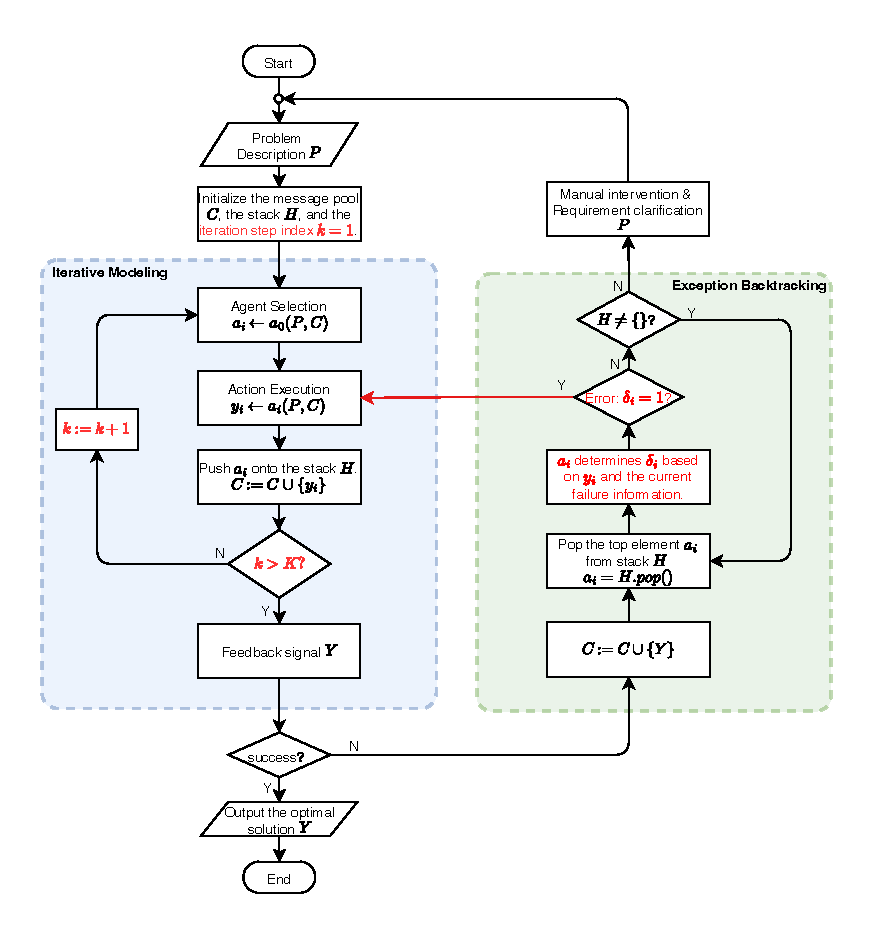
\includegraphics[scale=0.6]{sop_mas_flowchat_revise2.pdf}
\caption{Updated Figure~1 included for reviewer reference.}
\end{figure}



% ----------------------------------------------------------------------------
\subsection{Comment 3.8 and 3.9 --- Figure 2 Shows Wrong Problem (Airplane Landing, not ECR) \textbf{[COMPLETED]}}

\subsubsection{Comment}
\begin{enumerate}
\item \textbf{Comment 3.8: }``In lines 420-432 of section 3.4, the authors aim to describe the SOP-MAS process for a classic ECR case in container SCM using Figure 2. However, the figure actually represents the Aircraft Landing Problem. Additionally, the terms PD and MA agents are used instead of the previously established PM and BA.''
\item \textbf{Comment 3.9: }``Considering that Figure 2 is a crucial example of the framework, a more comprehensive explanation of the procedure illustrated in the figure would be beneficial and would greatly enhance readers' understanding. For instance, the exception backtracking component could be discussed in more depth within the content.''
\end{enumerate}

\subsubsection{Response}
We sincerely thank the reviewer for identifying this error. We acknowledge that Figure 2 inadvertently illustrated the Aircraft Landing Problem from the ComplexOR benchmark rather than the intended ECR case. This was a careless oversight during figure preparation. To produce an authentic illustration, we re-ran the SOP-MAS framework on a single-period, three-port ECR instance (ports A, B, C with supply $[100, 50, 0]$ and demand $[0, 0, 150]$ TEU) using the full five-agent configuration ($K{=}5$, with \texttt{is\_backward=True}). The system successfully solved the problem, obtaining an optimal objective value of ¥650, and all five agent outputs (DE-Agent through BA-Agent) were recorded. Figure 2 has been replaced with a new figure based on these actual outputs, with agent labels corrected to PM-Agent, DE-Agent, ME-Agent, PY-Agent, TE-Agent, and BA-Agent. Additionally, as suggested in Comment 3.9, we have expanded the explanation to include a dedicated paragraph describing the exception backtracking mechanism within the illustrative example.
\subsubsection{Modifications}
\begin{enumerate}
\item \textbf{Section 3.4 (Figure 2) --- REPLACE}
\begin{quote}
\textbf{Before:} ``\textit{Figure 2 illustrated the Aircraft Landing Problem with incorrect agent labels (PD, MA).}''\\[4pt]
\textbf{After:} ``\textit{\textcolor{red}{Figure 2 has been replaced with a correct ECR example showing the full SOP-MAS workflow on a three-port empty container repositioning problem, with agent labels corrected to PM-Agent, DE-Agent, ME-Agent, PY-Agent, TE-Agent, and BA-Agent.}}''
\end{quote}

\centering

\includegraphics[width=0.85\textwidth]{sop_mas_example.pdf}

\item \textbf{Section 3.4 (Figure caption) --- MODIFY}
\begin{quote}
\textbf{Before:} ``\textit{SOP-MAS Workflow Example}''\\[4pt]
\textbf{After:} ``\textit{\textcolor{red}{End-to-end SOP-MAS workflow on an ECR instance (3 ports, $T{=}1$): from natural-language description to optimal repositioning plan}}''
\end{quote}

\item \textbf{Section 3.4 (opening paragraph) --- REWRITE}
\begin{quote}
\textbf{Before:} ``\textit{In order to effectively demonstrate the capabilities of the proposed SOP-MAS workflow...a step-by-step exposition based on a classic case of ECR in container SCM is provided, as illustrated in Figure~2.}''\\[4pt]
\textbf{After:} ``\textit{\textcolor{red}{To demonstrate the end-to-end capability of the proposed SOP-MAS framework, we apply it to a single-period, three-port ECR instance. Ports A and B hold surplus containers (100 and 50 TEU, respectively) while port C demands 150 TEU; the unit transportation costs $c_{ij}$ range from 2 to 10 \textyen/TEU. The SOP-MAS is configured with $K{=}5$ collaborating agents, backtracking enabled, DeepSeek-V3-0324 as the backbone LLM, and Gurobi as the solver. The complete workflow is illustrated in Figure~2.}}''
\end{quote}

\item \textbf{Section 3.4 (agent walkthrough paragraph) --- REWRITE}
\begin{quote}
\textbf{Before:} ``\textit{The DE-Agent converts unstructured data and business constraints into consistent and reproducible modeling parameters... The ME-Agent automatically formulates a multi-period, multi-node mathematical model... The PY-Agent generates comprehensive, executable Python code... The TE-Agent executes the code within a sandboxed environment... The BA-Agent translates the model outputs...into an interpretable business-analysis report.}''\\[4pt]
\textbf{After:} ``\textit{\textcolor{red}{The PM-Agent orchestrates the five agents in sequence. First, the DE-Agent parses the natural-language problem description and extracts structured parameters: the supply vector $S{=}[100,50,0]$, the demand vector $D{=}[0,0,150]$, and the cost matrix $c_{ij}$. Second, the ME-Agent formulates the LP: $\min \sum_{i,j}c_{ij}x_{ij}$ subject to flow-balance constraints $\sum_j x_{ij}-\sum_j x_{ji}=S_i-D_i$ for each port $i$ and non-negativity $x_{ij}\geq 0$. Third, the PY-Agent generates executable Gurobi code implementing this model. Fourth, the TE-Agent executes the generated code with the actual input data, captures the solver log, and produces a structured diagnostic report; Gurobi solves the resulting LP in 2 iterations, yielding an optimal total repositioning cost of \textyen650. Fifth, the BA-Agent translates the optimal solution ($x_{AB}{=}50$, $x_{AC}{=}50$, $x_{BC}{=}50$) into a business-analysis report, identifying that the strategy routes surplus containers to the deficit port via the most cost-effective arcs.}}''
\end{quote}

\item \textbf{Section 3.4 (exception backtracking paragraph) --- ADD}
\begin{quote}
\textbf{After:} ``\textit{\textcolor{red}{Should an execution error or incorrect solution occur, the SOP-MAS framework triggers the exception backtracking mechanism. For instance, had the PY-Agent generated code that omitted a flow-balance constraint, the solver would report infeasibility, and the TE-Agent would capture the failure signal along with diagnostic evidence in the shared message pool. A stack-based reverse traversal is then performed: agents are popped in last-in-first-out order and each is queried to determine whether the error originated from its output. Upon locating the responsible agent, that agent provides a refined result, which is pushed back onto the stack, and the forward modeling resumes from the corrected step onward using the remaining collaboration rounds. This iterative correction loop continues until a valid solution is obtained or all collaboration rounds are exhausted.}}''
\end{quote}
\end{enumerate}

% ----------------------------------------------------------------------------
\subsection{Comment 3.10 --- Accuracy Increase Value Inconsistency \textbf{[COMPLETED]}}

\subsubsection{Comment}
``In line 501, the assertion `...realizing an increase in accuracy by 8.89\% over SPM' is inconsistent with the accuracy rates for COT and SPM, which are 52.26\% and 48.08\%, respectively. Consequently, the increase is not 8.69\%.''

\subsubsection{Response}
We verified the calculation: $(52.26-48.08)/48.08 = 8.69\%$, confirming the relative improvement is correct. To eliminate ambiguity between percentage-point differences and relative improvement, we revised the phrasing to explicitly state both values. During this revision, we conducted a self-audit of the entire manuscript and identified the same ambiguity pattern in Section 4.3 (ablation study), which has been corrected accordingly.

\subsubsection{Modifications}
\begin{enumerate}
\item \textbf{Section 4.1 (L423) --- MODIFY}
\begin{quote}
\textbf{Before:} ``\textit{realizing an increase in accuracy by 8.69\% over SPM}''\\[4pt]
\textbf{After:} ``\textit{realizing \textcolor{red}{an increase in accuracy from 48.08\% to 52.26\% (a relative improvement of 8.69\%)} over SPM}''
\end{quote}

\item \textbf{Section 4.3 (L484) --- MODIFY}
\begin{quote}
\textbf{Before:} ``\textit{there is a 28.75\% reduction in accuracy compared to the control group}''\\[4pt]
\textbf{After:} ``\textit{there is \textcolor{red}{a decrease in accuracy from 86.59\% to 57.84\%} compared to the control group}''
\end{quote}

\item \textbf{Section 4.3 (L484) --- MODIFY}
\begin{quote}
\textbf{Before:} ``\textit{a 13.42\% reduction in accuracy relative to the control group}''\\[4pt]
\textbf{After:} ``\textit{\textcolor{red}{a decrease in accuracy from 86.59\% to 73.17\%} relative to the control group}''
\end{quote}
\end{enumerate}

% ----------------------------------------------------------------------------
\subsection{Comment 3.11 --- \texttt{is\_backward} Formatting Inconsistency \textbf{[COMPLETED]}}

\subsubsection{Comment}
``In line 534, the phrase `...was deactivated (is\_backward = False)' should have `is\_backward = False' emphasized in bold, as it is in line 369.''

\subsubsection{Response}
We unified the formatting of \texttt{is\_backward} throughout the manuscript to use consistent monospace type.

\subsubsection{Modifications}
\begin{enumerate}
\item \textbf{Section 4.2 (L431) --- MODIFY}
\begin{quote}
\textbf{Before:} ``\textit{is\_backward=False}''\\[4pt]
\textbf{After:} ``\textit{\textcolor{red}{\texttt{is\_backward} = \texttt{False}}}''
\end{quote}
\end{enumerate}

% ----------------------------------------------------------------------------
\subsection{Comment 3.12 --- Symbols ``+'' and ``-'' Defined but Unused \textbf{[COMPLETED]}}

\subsubsection{Comment}
``In lines 581-582, the definitions of the symbols `+' and `-' are provided but are not applied anywhere in the manuscript.''

\subsubsection{Response}
We added the ``$+$'' and ``$-$'' symbols to the ablation table (Table~3) to annotate each group's backtracking status, making the symbols actionable and the table more self-contained.

\subsubsection{Modifications}

\begin{enumerate}
\item \textbf{Table 3 (L473--478) --- MODIFY}
\begin{quote}
\textbf{Before:} ``\textit{Group1, Group2, Group3, Group4, Group5, Control Group}''\\[4pt]
\textbf{After:} ``\textit{\textcolor{red}{Group1 ($-$), Group2 ($+$), Group3 ($+$), Group4 ($+$), Group5 ($-$), Control Group ($+$)}}''
\end{quote}
\end{enumerate}

% ----------------------------------------------------------------------------
\subsection{\textbf{[COMPLETED]} Comment 3.13 --- $S_i^t$ Variable $t$ Undefined}

\subsubsection{Comment}
``In line 689, the variable `$t$' within `$S_i^t$' lacks a definition.''

\subsubsection{Response}
We thank the reviewer for identifying this omission. The time period index $t$ was indeed used without prior definition in the problem description. We have added an explicit definition of the time period set $T$ and index $t \in T$ at the beginning of Section~5.2. Furthermore, upon systematic inspection prompted by this comment, we discovered that the ECR model notation (Sections~5.2 and Appendix~C) shared several symbols with the SOP-MAS methodology (Section~3), including $H$ (backtracking stack vs.\ seaport set), $K/k$ (agent iteration steps vs.\ transport modes), $S$ (state variable vs.\ supply), and $y$ (agent output vs.\ rental quantity). To eliminate all ambiguities, we have comprehensively redesigned the ECR notation using a three-tier convention (calligraphic capitals for sets, uppercase Romans for parameters, lowercase Romans for decision variables) while keeping Section~3 unchanged. The complete mapping is provided in the Modifications subsection below.

\subsubsection{Modifications}

\begin{enumerate}
\item \textbf{Section 5.2, Problem Description (line 536) --- ADD}
\begin{quote}
\textbf{After:} ``\textit{such that $\mathcal{N}=\mathcal{P}\cup\mathcal{L}$. \textcolor{red}{Let $T=\{1,2,\ldots,|T|\}$ denote the set of time periods in the planning horizon, indexed by $t \in T$.} The collection of edge $E$ symbolizes}''
\end{quote}

\item \textbf{Section 5.2 + Appendix C --- MODIFY (Notation Harmonization)}
\begin{quote}
To eliminate all symbol conflicts with the SOP-MAS methodology (Section 3), the ECR model notation has been systematically redesigned as follows:

\begin{tabular}{lll}
\toprule
\textbf{Old Symbol} & \textbf{New Symbol} & \textbf{Meaning} \\
\midrule
$H$ & \textcolor{red}{$\mathcal{P}$} & Seaport set \\
$L$ & \textcolor{red}{$\mathcal{L}$} & Dry port set \\
$N=H\cup L$ & \textcolor{red}{$\mathcal{N}=\mathcal{P}\cup\mathcal{L}$} & Node set \\
$K$ & \textcolor{red}{$\mathcal{M}$} & Transport mode set \\
$k$ & \textcolor{red}{$m$} & Transport mode index \\
$S_i^t$ & \textcolor{red}{$Q_i^t$} & Empty container supply \\
$y_i^t$ & \textcolor{red}{$r_i^t$} & Rental quantity \\
\bottomrule
\end{tabular}
\end{quote}
\end{enumerate}

% ----------------------------------------------------------------------------
\subsection{\textbf{[COMPLETED]} Comment 3.14 --- ECR Case Solution Lacks Numerical Evidence}

\subsubsection{Comment}
\begin{enumerate}
\item \textbf{Comment 3.14: }``In lines 719-729, the solution derived from the SOP-MAS framework is presented, yet the discussion lacks supporting numerical evidence. Including a more comprehensive discussion with examples would significantly enhance the paper's quality.''

\item \textbf{Comment 3.15: }``In line 745, the mention of the reduction in repositioning cost as a percentage appears abruptly in the conclusion. This improvement should be addressed in Section 5.3, where the model's solution is analyzed.''
\end{enumerate}

\subsubsection{Response}
We thank the reviewer for this constructive suggestion. The original Section 5.3 contained only qualitative descriptions without specific numerical results. We have substantially revised this section by (1) reporting the optimal objective value and cost breakdown for Scenario~1 (sea–land coordination), (2) adding a detailed cost comparison table between the two scenarios with percentage changes, and (3) providing concrete numerical evidence for each qualitative claim. Additionally, we corrected a misstatement in the Conclusion: the 12.18\% reduction refers to total operational costs, not repositioning costs alone.

\subsubsection{Modifications}

\begin{enumerate}
\item \textbf{Section 5.3, Results Analysis (lines 548--552) --- MODIFY}
\begin{quote}
\textbf{Before:} ``\textit{To evaluate the benefits of the sea--land intermodal transport mode, a comparative analysis was conducted under the scenario wherein dry ports are unable to facilitate the exchange of empty containers among themselves, as illustrated in Figure~5. The results show that the repositioning of empty containers from dispersed dry ports to seaports experiencing shortages becomes increasingly challenging. Consequently, there is an increase in both the volume of empty containers transported directly from dry ports to seaports and the volume circulated among seaports, ultimately leading to elevated overall costs. Furthermore, the exacerbated difficulty in empty container flows leads to a greater number of containers failing to arrive at shortage seaports in a timely manner, which in turn increases the leasing demand at the affected seaports and significantly escalates repositioning costs.}''\\[4pt]
\textbf{After:} ``\textit{\textcolor{red}{Under the sea--land coordination scenario (Scenario~1), wherein hinterland lateral repositioning is permitted, the optimal total cost over the five-period planning horizon is CNY~1,190,336, comprising repositioning costs of CNY~763,966, holding costs of CNY~30,870, and leasing costs of CNY~395,500, as summarized in Table~6.}} \textcolor{red}{To evaluate the benefits of hinterland lateral repositioning, a comparative analysis was conducted under the scenario without inter-dry-port exchange (Scenario~2), as illustrated in Figure~5. As shown in Table~6, the total cost increases from CNY~1,190,336 to CNY~1,355,388 (+13.86\%). This increase is primarily driven by the repositioning costs, which rise from CNY~763,966 to CNY~925,238 (+21.11\%). Within the repositioning category, the sea--land repositioning cost surges from CNY~594,952 to CNY~864,910 (+45.38\%), as the network must compensate for the loss of hinterland lateral flows (CNY~110,718 reduced to zero) by routing more containers through the sea--dry corridors. Furthermore, the exacerbated difficulty in empty container flows leads to a greater number of containers failing to arrive at shortage seaports in a timely manner, which in turn increases the leasing demand at the affected seaports from CNY~395,500 to CNY~406,000 (+2.66\%). Overall, enabling hinterland lateral repositioning yields a 12.18\% reduction in total operational costs.}''
\end{quote}

\item \textbf{Section 5.3 --- ADD (New Table)}
\begin{quote}
\textbf{After:} A new table (Table: Cost comparison between the two scenarios) has been inserted in Section~5.3, presenting a seven-row cost breakdown comparing Scenario~1 and Scenario~2 across repositioning sub-categories, holding, leasing, and total costs, with percentage changes for each row.
\end{quote}

\item \textbf{Section 6, Conclusions (line 571) --- MODIFY}
\begin{quote}
\textbf{Before:} ``\textit{leading to a 12.18\% reduction in repositioning costs for the shipping company.}''\\[4pt]
\textbf{After:} ``\textit{leading to a 12.18\% reduction in \textcolor{red}{total operational costs} for the shipping company (see Table 6 for details).}''
\end{quote}
\end{enumerate}


% ----------------------------------------------------------------------------
\subsection{Comment 3.16 --- Future Research Directions in Conclusion \textbf{[COMPLETED]}}

\subsubsection{Comment}
``In the concluding section, it would be advantageous to explore potential future research directions. Given the rapid development and interest in this area of operations research, such a discussion would be a valuable addition.''

\subsubsection{Response}
We thank the reviewer for this constructive suggestion. We have restructured the concluding section to include a dedicated discussion of future research directions. Rather than appending a separate paragraph, we integrated the future directions organically into the existing conclusion by replacing the previously scattered outlook statements with a coherent, structured discussion covering three key avenues: extending to more complex optimization paradigms, fine-tuning domain-specific LLMs, and deploying in human-in-the-loop settings.

\subsubsection{Modifications}

\begin{enumerate}
\item \textbf{Section~Conclusions (line~597) --- MODIFY}
\begin{quote}
\textbf{Before:} ``\textit{As training parameters and scale increase, pre-trained LLMs are anticipated to achieve further advancements in capability. By integrating general-purpose LLMs with customized knowledge bases, the cost associated with decision-making can be significantly reduced. From the perspective of shipping companies, which occupy a central role in the empty container repositioning process, the proposed approach can be further extended to support additional stakeholders, including seaports, dry ports/inland container yards, shippers/customers, and third-party leasing companies.}''\\[4pt]
\textbf{After:} ``\textit{\textcolor{red}{Several promising directions merit further investigation. First, extending the framework to more complex optimization paradigms, such as stochastic programming, robust optimization, and multi-objective optimization, would broaden its applicability to real-world ECR scenarios involving uncertainty and conflicting objectives. Second, fine-tuning domain-specific LLMs on curated OR problem--solution pairs presents an opportunity to enhance both modeling performance and computational efficiency. Third, deploying the framework in interactive, human-in-the-loop settings would enable iterative refinement based on practitioner feedback, while extending its scope to support additional stakeholders, such as seaports, dry ports, shippers, and third-party leasing companies, in the broader container SCM.}}''
\end{quote}
\end{enumerate}
% ----------------------------------------------------------------------------
\subsection{Comment 3.17 --- Move Math Model from Appendix to Main Text}

\subsubsection{Comment}
``A minor suggestion: the authors might consider integrating the mathematical programming model for the problem into the main body of the paper, rather than relegating the LaTeX version to the appendix. While it is understandable that the authors aim to highlight the results from the LLM and MAS approach, this presentation may complicate the understanding of the problem and model. However, it is understandable if the authors choose to retain the model in its current LaTeX format.''

\subsubsection{Response}

\subsubsection{Modifications}

\end{document}
